\begin{frame}
\frametitle{Creare Una Swapchain}
\begin{columns}

\column{.6\textwidth}

\begin{itemize}
\item Una volta creato un device logico, lo possiamo utilizzare per creare una swapchain
\item Dobbiamo creare una swapchain per presentare immagini sulla presentation surface
\item Una swapchain crea e gestisce le immagini che saranno presentate
\item Tramite la swapchain dobbiamo specificare la modalità di presentazione che verrà usata dal presentation engine del sistema operativo
\end{itemize}

\column{.2\textwidth}

\begin{figure}[ht]
    \centering
    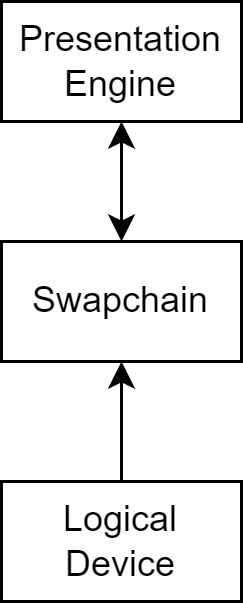
\includegraphics[scale=0.2]{images/SlidesInitializingVulkan/Swapchain.png}
\end{figure}

\end{columns}
\end{frame}
